\documentclass[conference]{IEEEtran}

\usepackage{cite}
\usepackage{amsmath,amssymb,amsfonts}
\usepackage{graphicx}
\usepackage{booktabs}
\usepackage{textcomp}
\usepackage{xcolor}
\usepackage{url}

\begin{document}

\title{Inferring Latent Bitcoin Market Regimes with Hidden Markov Models}

\author{
\IEEEauthorblockN{Muzzammil Soofie}
\IEEEauthorblockA{
School of Computer Science and Applied Mathematics\\
University of the Witwatersrand\\
Johannesburg, South Africa\\
your.email@students.wits.ac.za
}
}

\maketitle

\begin{abstract}
This paper investigates whether hidden Markov models can infer meaningful latent Bitcoin market regimes from weekly market observations. The study compares price-only, macro, trader-style technical, and psychology-enhanced feature families. The strongest model combines price information with psychology-linked variables, including the Crypto Fear and Greed Index, momentum, and drawdown. Results suggest that psychology-linked features improve regime inference more than macro-only and trader-only feature sets in this weekly setting. The inferred regimes are economically interpretable and align with neutral or recovery, greed or bull, and fear or stress market conditions. Additional evaluation against simple baselines and a masked-feature recovery test supports the usefulness of temporal latent-state modeling for short-term Bitcoin regime analysis.
\end{abstract}

\begin{IEEEkeywords}
Hidden Markov Model, Bitcoin, market regimes, sentiment, behavioral finance, time series
\end{IEEEkeywords}

\section{Introduction}
Bitcoin exhibits large shifts in volatility, trend, and market sentiment. Many forecasting approaches attempt to predict the next return directly, but such models often provide limited insight into the latent state of the market. This paper instead models Bitcoin as a sequence of hidden regimes, where each regime generates different observable patterns in return, volatility, trading activity, and psychology-linked indicators.

The main goal is to test whether an HMM can infer meaningful latent Bitcoin regimes and whether psychology-linked variables improve regime inference relative to price-only, macro, and trader-style technical indicators. A second goal is to evaluate whether the inferred regimes support short-term directional prediction and masked-feature recovery.

The main contributions of this work are:
\begin{itemize}
    \item a weekly Bitcoin HMM framework for latent regime inference;
    \item a comparison of five feature families;
    \item baseline comparisons against non-HMM methods;
    \item a cover-up evaluation in which known features are masked and reconstructed.
\end{itemize}

\section{Data and Feature Families}
The dataset uses weekly observations constructed from daily data beginning in February 2018. Core market variables include Bitcoin log return, rolling volatility, and volume change. Additional feature families were designed to test distinct sources of information:

\begin{itemize}
    \item \textbf{Price only:} return, volatility, and volume change.
    \item \textbf{Price + psychology:} price variables plus Fear and Greed, momentum, and drawdown.
    \item \textbf{Price + macro:} price variables plus dollar index return and 10-year yield change.
    \item \textbf{Price + trader:} price variables plus moving-average spread and price relative to a longer moving average.
    \item \textbf{Compact combined:} a smaller mixed feature set spanning multiple families.
\end{itemize}

Weekly frequency was used to reduce noise and better align slower-moving sentiment and macro-financial variables with Bitcoin market behavior.

\section{Methodology}
Let $z_t$ denote the hidden market regime at week $t$ and let $x_t$ denote the observed feature vector. The HMM assumes a first-order Markov structure over hidden states and regime-conditional emissions over observations:
\begin{equation}
P(z_{1:T}, x_{1:T}) = P(z_1)\prod_{t=2}^{T} P(z_t \mid z_{t-1}) \prod_{t=1}^{T} P(x_t \mid z_t).
\end{equation}

Gaussian HMMs with diagonal covariance were fitted using multiple random restarts. Both three-state and four-state models were tested. The study used a chronological train-test split so that later weeks were never used during training. Feature scaling was applied using training data only.

After fitting, the most likely hidden-state sequence was decoded and each state was interpreted using its average return, volatility, sentiment, momentum, and drawdown characteristics.

\section{Evaluation Protocol}
Evaluation was intentionally broad because a regime model should be judged on more than one metric.

\subsection{Feature-family comparison}
Each feature family was evaluated under three-state and four-state configurations using out-of-sample accuracy and balanced accuracy for next-week direction.

\begin{table}
\caption{Best-performing HMM configuration within each feature family (out-of-sample test set).}
\label{tab:feature_families}
\begin{tabular}{lrrrr}
\toprule
Feature family & Features & States & Accuracy & Balanced accuracy \\
\midrule
Price only & 3 & 4 & 0.548 & 0.530 \\
Price + psychology & 6 & 3 & 0.583 & 0.572 \\
Price + macro & 5 & 3 & 0.464 & 0.467 \\
Price + trader & 5 & 4 & 0.500 & 0.505 \\
Compact combined & 7 & 3 & 0.548 & 0.500 \\
\bottomrule
\end{tabular}
\end{table}


\subsection{Baseline comparison}
The best HMM was compared against a majority-class rule, a last-sign rule, logistic regression, and a Gaussian mixture model. This comparison tests whether temporal latent-state modeling adds value beyond static clustering or simple discriminative prediction.

\begin{table}
\caption{Comparison against non-HMM baselines.}
\label{tab:baselines}
\begin{tabular}{lrrr}
\toprule
Model & Accuracy & Balanced accuracy & Features \\
\midrule
Majority class & 0.548 & 0.500 & NaN \\
Last sign & 0.524 & 0.519 & NaN \\
Logistic regression & 0.524 & 0.535 & 6.000 \\
GMM (3 clusters) & 0.548 & 0.543 & 6.000 \\
HMM psychology (3 states) & 0.583 & 0.572 & 6.000 \\
\bottomrule
\end{tabular}
\end{table}


\subsection{Cover-up testing}
A masked-feature recovery experiment was used as a generative evaluation. Selected psychology-linked variables were hidden on the test set and reconstructed using HMM state-conditioned means estimated from training data. Performance was compared against a simple global-mean baseline using MAE and RMSE.

\begin{table}
\caption{Masked-feature recovery on the test set using HMM state-conditioned reconstruction versus a global-mean baseline.}
\label{tab:coverup}
\begin{tabular}{lrrrr}
\toprule
Masked feature & HMM MAE & Mean MAE & HMM RMSE & Mean RMSE \\
\midrule
Fear \& Greed & 15.440 & 19.964 & 18.467 & 22.543 \\
4-week momentum & 0.092 & 0.094 & 0.109 & 0.129 \\
12-week drawdown & 0.077 & 0.102 & 0.093 & 0.111 \\
\bottomrule
\end{tabular}
\end{table}


\section{Results and Analysis}
The strongest feature family was the psychology-enhanced model, and the best configuration within that family used three latent states. These states can be interpreted as:
\begin{itemize}
    \item \textbf{Neutral or recovery:} near-flat return, moderate sentiment, shallow drawdown;
    \item \textbf{Greed or bull:} high positive return, high Fear and Greed, strong momentum, minimal drawdown;
    \item \textbf{Fear or stress:} negative return, low Fear and Greed, negative momentum, deep drawdown.
\end{itemize}

The state transition structure was also realistic. The fear or stress state was highly persistent, the neutral or recovery state was moderately persistent, and direct transition from bull to fear was effectively absent, suggesting a more plausible bull-to-neutral-to-fear dynamic than a purely static clustering model.

\begin{figure}[t]
    \centering
    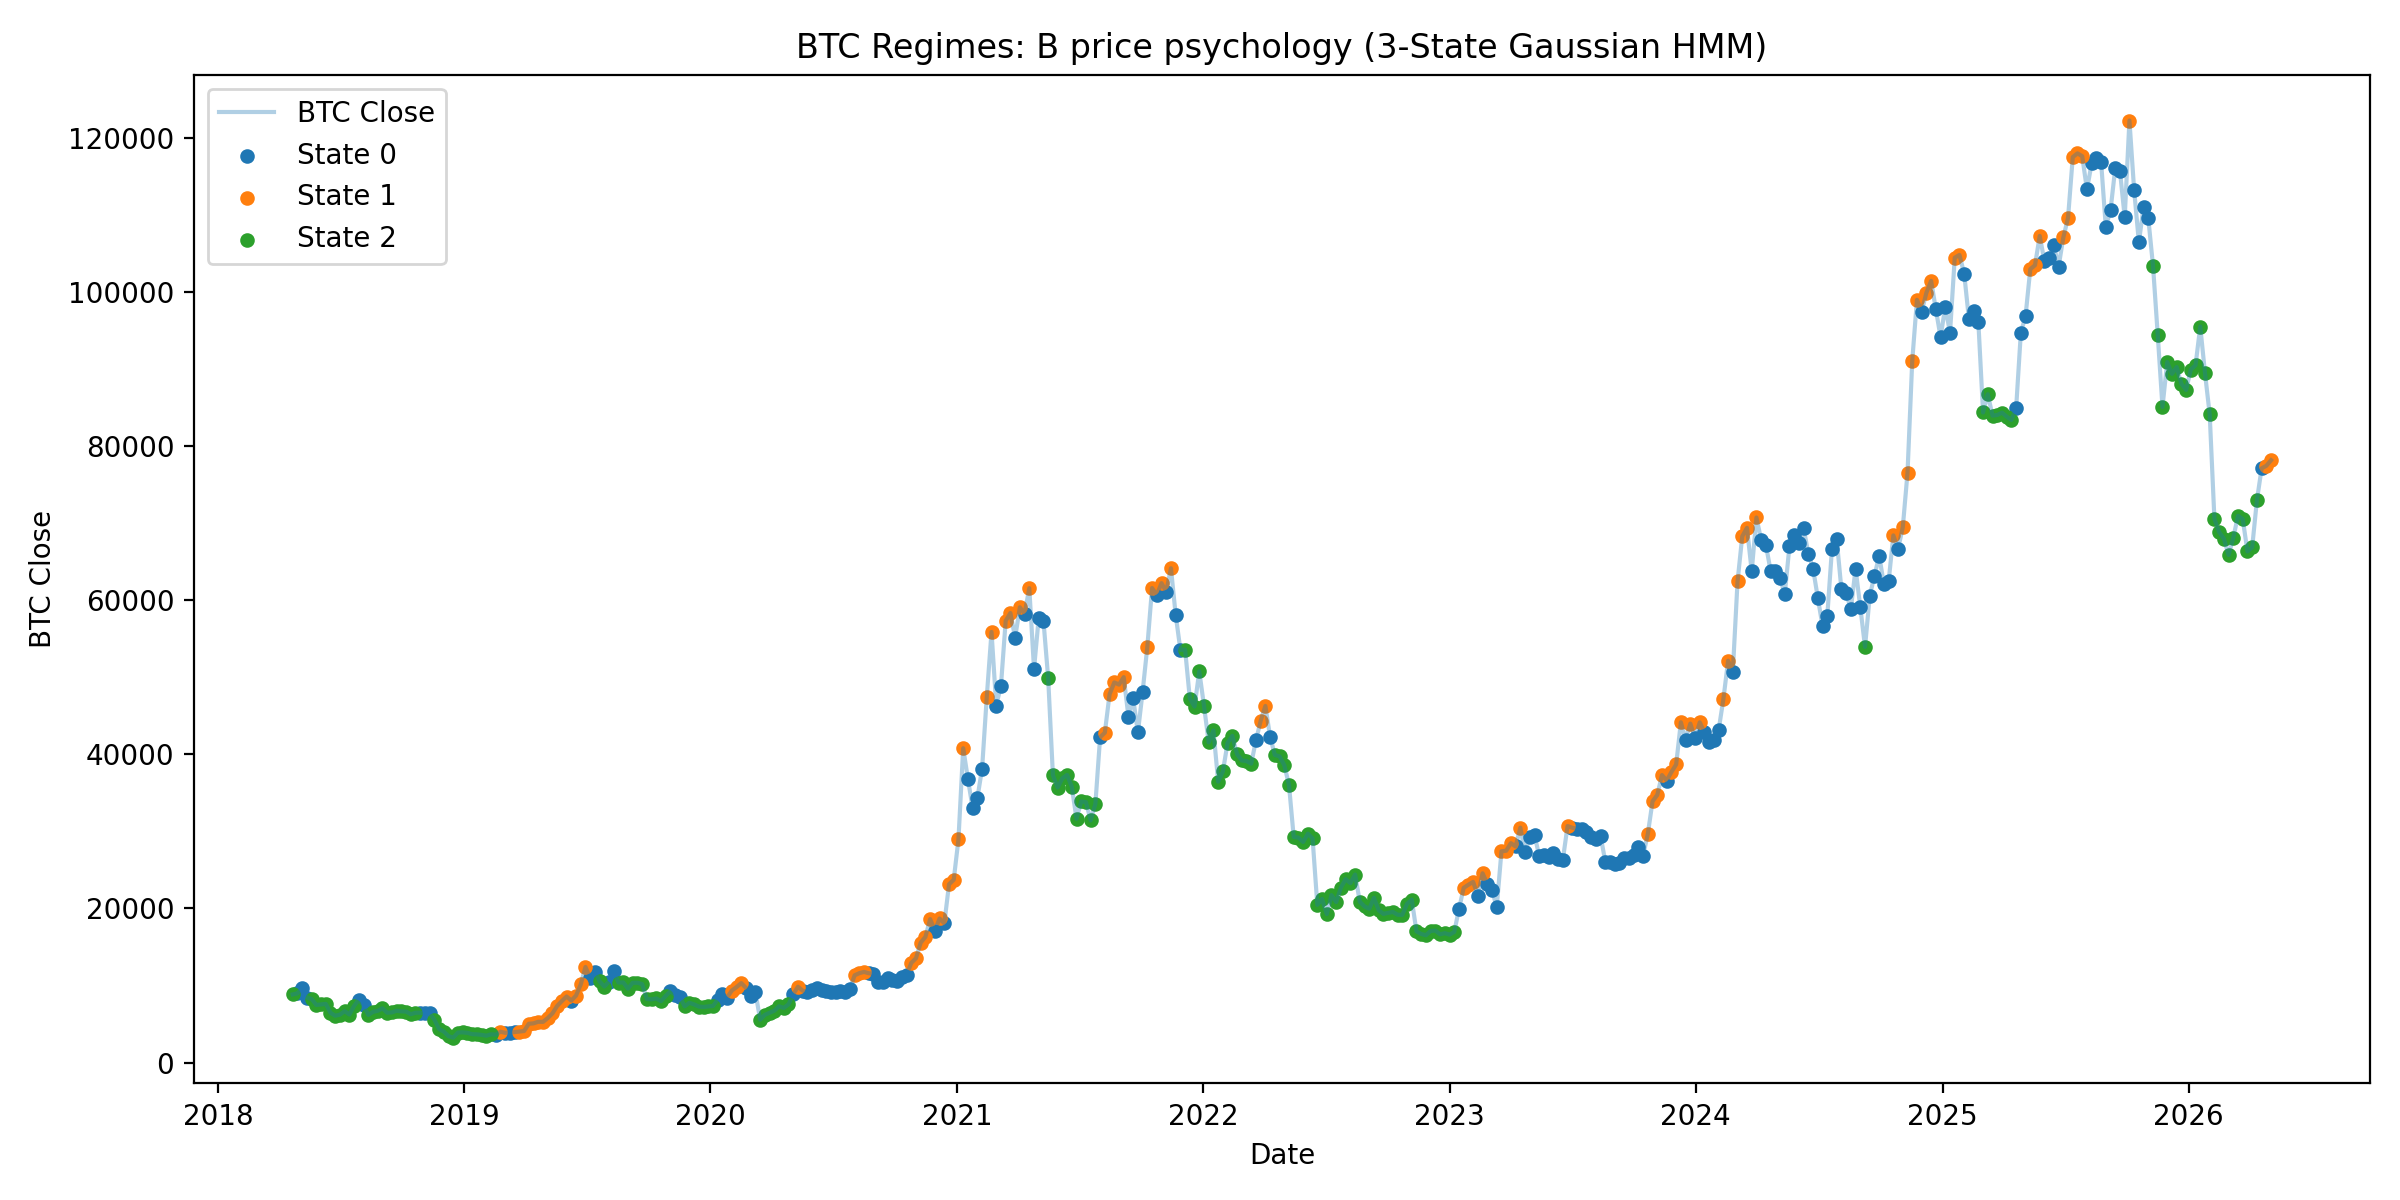
\includegraphics[width=\columnwidth]{../results/figures/B_price_psychology_btc_regimes_3_states.png}
    \caption{Bitcoin closing prices with decoded states from the best-performing three-state psychology-enhanced HMM.}
    \label{fig:psychology_regimes}
\end{figure}

The baseline comparison showed that the HMM outperformed the majority-class baseline, the last-sign baseline, logistic regression, and a Gaussian mixture model on the same psychology-linked features. This suggests that both temporal structure and latent-state modeling contributed useful information beyond static clustering and direct classification.

The cover-up testing results further support the model. When Fear and Greed, momentum, or drawdown were masked, the HMM-based reconstruction outperformed a global-mean baseline. This indicates that the learned hidden states captured meaningful joint structure among the psychology-linked variables.

\section{Discussion}
The main finding is that psychology-linked variables were more useful than macro-only or trader-only feature families for this weekly Bitcoin regime-inference task. This result supports the idea that Bitcoin market dynamics may be more strongly tied to behavioral and sentiment-like cycles than to the limited macro-financial inputs used here.

The trader-style feature family was not dominant on its own, but it still provided an informative comparison against the types of indicators commonly used by retail traders. The macro-only family performed poorly in this setting, which may reflect limited sample size, weak weekly alignment, or insufficient macro coverage rather than the complete irrelevance of macro conditions.

A limitation of the approach is the Gaussian emission assumption. Bitcoin returns are heavy-tailed, so some extreme episodes may be represented imperfectly. Another limitation is data size, since the sentiment history constrains the available weekly sample. Future work could test richer sentiment inputs, alternative emission models, or longer-horizon prediction tasks.

\section{Conclusion}
This paper presented an HMM-based approach for inferring latent Bitcoin market regimes from weekly data. Among the compared feature families, a psychology-enhanced HMM achieved the strongest out-of-sample performance and yielded clear market-psychology interpretations. The results suggest that latent-state modeling with psychology-linked features is a promising way to study Bitcoin market structure and short-term regime behavior.

\section*{Acknowledgment}
Remove this section if not needed.

\begin{thebibliography}{00}

\bibitem{placeholder1}
Placeholder reference 1.

\bibitem{placeholder2}
Placeholder reference 2.

\bibitem{placeholder3}
Placeholder reference 3.

\end{thebibliography}

\end{document}